\documentclass[10pt,a4paper]{article}
\usepackage[utf8]{inputenc}
\usepackage[francais]{babel}
\usepackage[T1]{fontenc}
\usepackage{amsmath}
\usepackage{amsfonts}
\usepackage{amssymb}
\usepackage{kpfonts}
\usepackage{pdfpages}
%\author{Mathieu Leocmach}
\title{Rapport de jury de thèse}
\date{}
\begin{document}
\maketitle
\textit{Traduction du japonais par le candidat lui-même. Aucune liste signée des membres du jury n'est délivrée par l'université de Tokyo. Les diplômes japonais ne comportent pas de mention. Veuillez trouver le document original en pages 3-4.}

\bigskip

\begin{description}
\item[Titre de la thèse] Hétérogénéités structurales et dynamiques des liquides colloïdaux surfondus : étude par microscopie confocale
\item[Nom du candidat] LEOCMACH Mathieu
\end{description}

\bigskip

La thèse porte sur la dynamique lente de dispersions colloïdales (système de sphères dures) proches de la transition vitreuse. Une technique de microscopie confocale permet de localiser et suivre le mouvement des particules individuelles afin d'exposer les causes structurelles de la dynamique lente.

\bigskip

Dans le chapitre 1, est exposé le contexte et l'objet de la recherche. La transition vitreuse est encore un phénomène mystérieux lors duquel le temps de relaxation du liquide surfondu augmente de plus de 10 ordres de grandeur malgré peu de changement dans la fonction de corrélation de la densité. De plus, des hétérogénéités transitoires de la dynamique ont été mises en évidence au sein du liquide surfondu. Le lien entre ces deux phénomènes reste un problème ouvert.
Sont abordés également des exemples de recherches récentes à propos de la relation entre les hétérogénéités statique et dynamique. L'objectif central de cette thèse est d'examiner cette relation entre la structure et la dynamique afin de découvrir l'origine physique de la dynamique lente associée à la transition vitreuse.

Dans le chapitre 2, est exposé le procédé de synthèse des colloïdes marqués par fluorescence utilisés dans les expériences, le principe de la microscopie confocale à balayage laser en trois dimensions et les détails expérimentaux comme la façon d'accorder en densité et en indice de réfraction les particules avec leur solvant. Au chapitre 3, est exposée une nouvelle méthode de localisation rapide de particules. Le chapitre 4 se concentre sur l'analyse quantitative de la structure locale. Le chapitre 5 expose les méthodes d'accélérations de ces traitements de données.

Dans le chapitre 6 sont décrits les détails des résultats expérimentaux dans une suspension colloïdale polydispersée (6\% de polydispersité). La dépendance de la structure du liquide en fonction de la fraction volumique est analysée à l'approche de la transition vitreuse. Les structures jouant un rôle majeur sont identifiées comme d'une part un ordre de lien local cristallin (des clusters de durée de vie comparables au temps de relaxation du système et présentant une symétrie locale proche de celle du cristal) et d'autre part un ordre de lien icosaédrique. En évaluant directement la durée de vie et la taille de ces deux structures il est montré que l'ordre pseudo-cristallin (longue durée de vie, étendu spatialement) joue un rôle plus important que les icosaèdres (de durée de vie relativement courte et spatialement isolés). L'analyse quantitative de la géométrie local indique que la stabilité des icosaèdres est due au volume plus important disponible pour la particule centrale ce qui contribue à augmenter l'entropie du système. Par conséquent, l'ordre pseudo-cristallin et l'ordre icosaédrique augmentent tous deux l'entropie du système, abaissant ainsi l'énergie libre, ce qui justifie leur existence et leur stabilité dans le liquide surfondu.

Le chapitre 7 contient les résultats d'une étude sur la dynamique de la nucléation hétérogènes de cristaux et leur croissance à la proximité d'une paroi du récipient contenant le système (même dispersion colloïdale à 6\% de polydispersité). Des icosaèdres sont détectées au voisinage de l'interface entre les cristaux et le liquides, ce qui est présenté comme une frustration à l'encontre du processus de cristallisation. Au chapitre 8, une analyse quantitative de la dynamique des particules du liquide en surfusion permet de discuter de la corrélation entre la structure locale et la dynamique locale. Le chapitre 9 est un résumé de l'ensemble.

\bigskip

Il est démontré qu'il existe un lien fort entre la structuration locale et la lenteur de la dynamique. En évaluant indépendamment les longueurs de corrélation structurelle et dynamique, il est montré que toutes deux varient de concert en suivant la même dépendance en fraction volumique, divergeant à l'approche de la transition vitreuse idéale, ce qui rappel fortement les phénomènes critiques. Jusqu'à présent, dans le contexte de la dynamique lente des liquides surfondus, l'importance de la structure locale avait été proposée dans le laboratoire de la thèse par des simulations et des théories, pourtant il n'y avait aucune preuve expérimentale directe. Justement la présente étude, grâce à des mesures directes de la position de chaque particule, démontre expérimentalement pour la première fois qu'il existe une très forte corrélation entre un ordre orientationnel local et la dynamique. En particulier, il est clairement démontré pour la première fois dans la présente étude que, tout au moins dans les systèmes de verres colloïdaux, c'est l'ordre pseudo cristallin (frustré par les icosahèdres) et non l'ordre icosaédrique (localement stable, mais frustré par son incapacité à paver l'espace) qui est la clé de la dynamique lente. Il est montré que la structure icosaédrique, au lieu de provoquer directement le ralentissement de la dynamique, agit comme un facteur de frustration inhibant la cristallisation.

\bigskip

Comme mentionné plus haut, les résultats obtenus dans la présente étude amènent le point de vue original de la structure locale du liquide sur le problème, non résolu depuis de nombreuses années et extrêmement important du point de vue de la physique appliquée, de l'origine de la dynamique lente associée à la transition vitreuse. En conséquence, le candidat a été déclaré digne du titre de docteur (ingénierie).

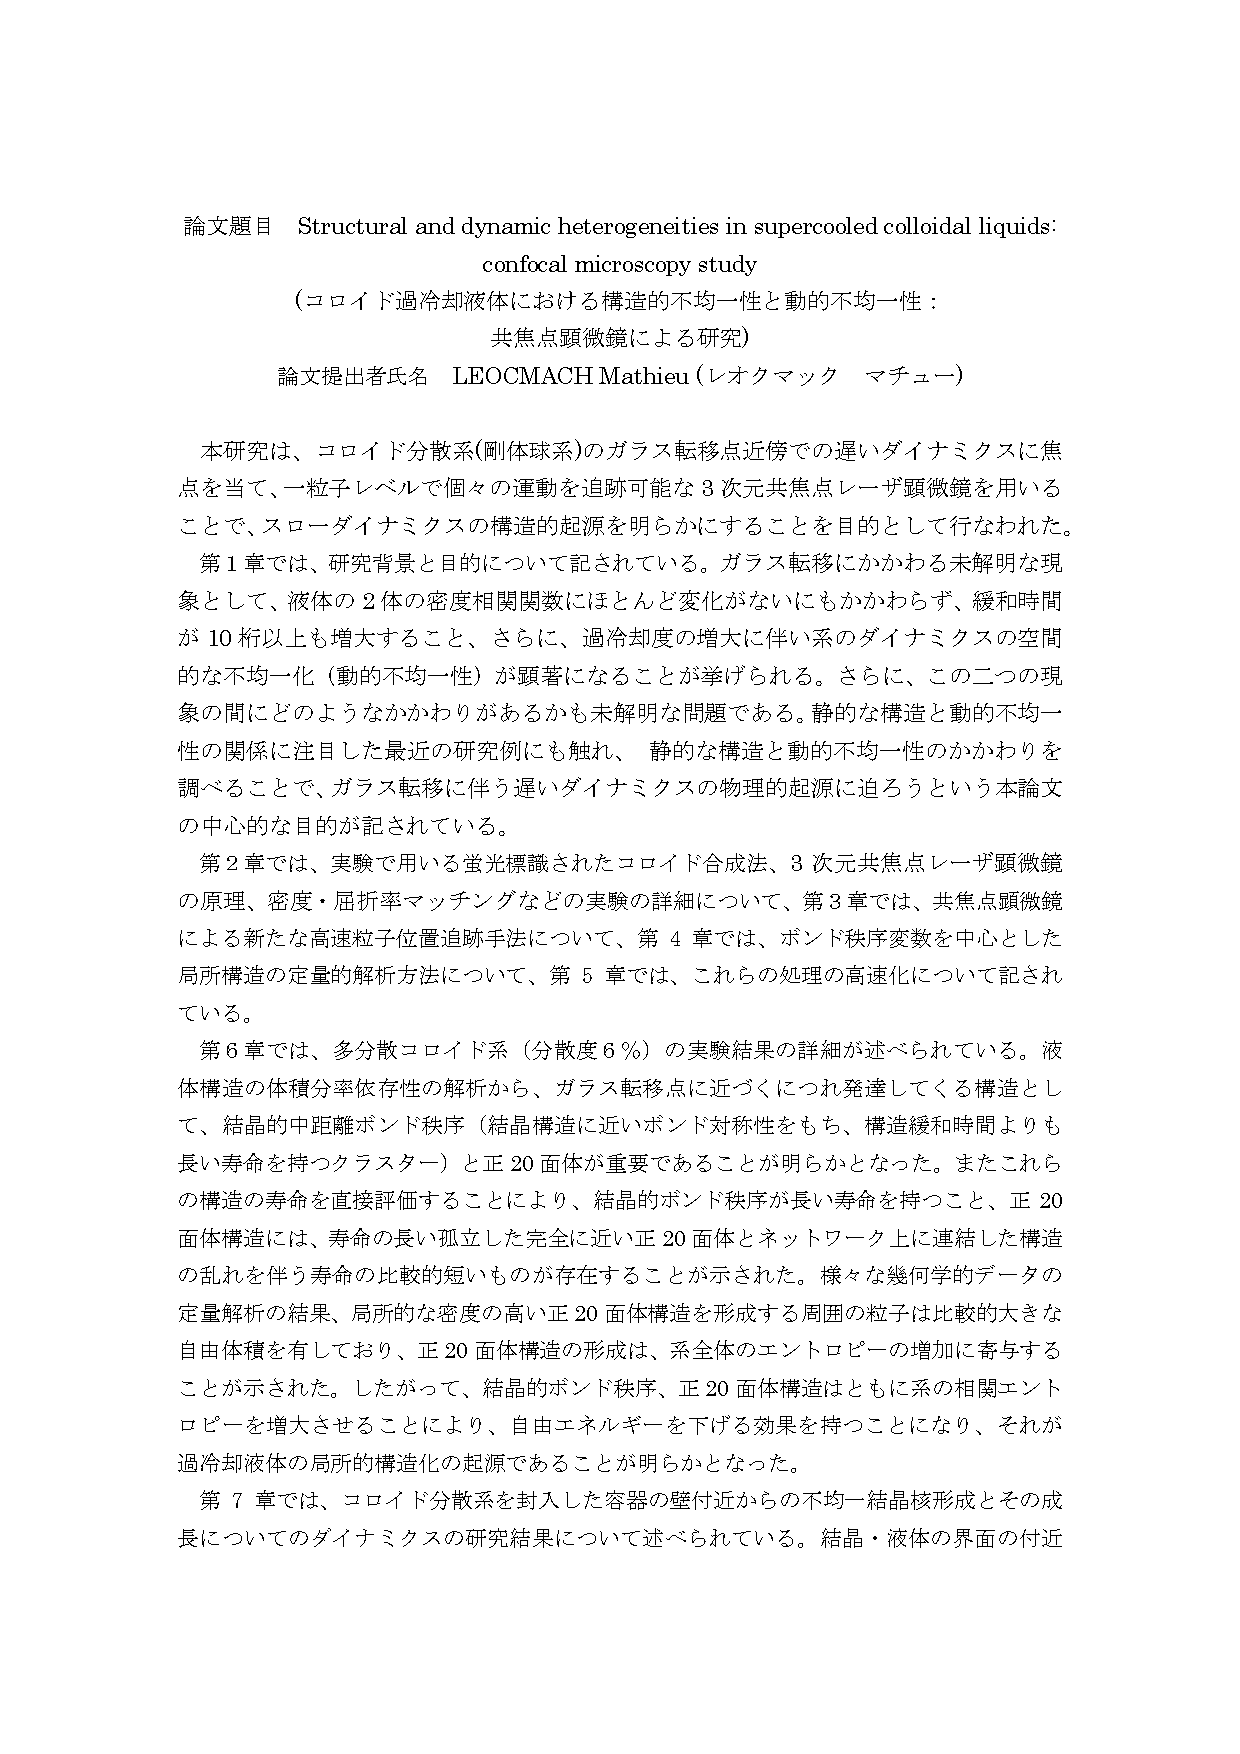
\includepdf[pages={1-},scale=1]{hakaseshinsayoushi(Leocmach).pdf}
\end{document}